\documentclass{article}
\usepackage[utf8]{inputenc}
\title{Video 3: The Law of Large Numbers and Deviation Inequalities}
\author{wbg231 }
\date{December 2022}
\newcommand{\R}{$\mathbb{R}$}
\newcommand{\B}{$\beta$}
\newcommand{\A}{$\alpha$}
\newcommand{\D}{\Delta}

\newcommand{\avector}[2]{(#1_2,\ldots,#1_{#2})}
\newcommand{\makedef}[2]{$\textbf{#1}$:#2 }
\usepackage{tikz,graphicx,hyperref,amsmath,amsfonts,amscd,amssymb,bm,cite,epsfig,epsf,url}

\begin{document}

\maketitle

\section{introduction}
\begin{itemize}
\item \href{https://www.youtube.com/watch?v=MmqywUdajQs&list=PLBEf5mJtE6KuZ5NBQMuWIMsiOOrV9ibzm&index=68}{video link}
\item today we are talking about law of large numbers
\item the law of large numbers tells us that when we average a large number of random variables with the same mean and finite variance there average converges to the mean of the distribution, this justifies using sample mean to estimate population mean 
\item in a way we have come full circle because we defined the mean of a random viable as representing samples from the co responding distribution of the random variable, so under the right assumptions this definition will give us a good estimator of the mean 
\item motivation is the estimation of population parameters. ie we want to estimate some population parameter using a limited quantity of data. 
\item the sample mean is a random variable so we need to analyze the estimator in a  probabilistic way
\section{sample mean review/set up }
\item let the population parameter we are looking for be the population mean $\mu_{pop}$
\item let the population variance be $\sigma^2_{pop}$
\item  random samples are selected independent and uniformly at random with replacement $\Tilde{x}_{1}...\Tilde{x}_{n}$
\item $\Tilde{m}=\frac{1}{n}\Sigma_{i=1}^{n}\Tilde{x}_{i}$
\item and the sample mean is unbiased that is $E[\Tilde{m}]=\mu_{pop}$
\item we further showed that the standard error which is the standard deviation of the same mean is $se[\Tilde{m}]=\frac{\sigma_{pop}}{\sqrt{n}}$ which is inversely proportional to the sample size, meaning as the sample grows our sample means become more tightly packed around the population mean which is what we are trying to estimate
\item as we increase n we can see this behavior happen 
\section{convergence in mean square}
\item consider independent random variables $\Tilde{x}_1,\Tilde{x}_2,\Tilde{x}_3....$ (that is an infinite sequence of independent random variables) all with mean finite $\mu$ and finite variance $\sigma^2$ (so these are an infinite number of random warbles representing draws from the population)
\item so call the running mean of that $\Tilde{m}_{n}=\frac{1}{n}\Sigma_{j=1}^{n}\Tilde{x}_j$ this is the same as taking random samples from a population
\item if we look at the mean of this running average we can see that $E[\Tilde{m}_{n}]=E[\frac{1}{n}\Sigma_{j=1}^{n}\Tilde{x}_j]=\frac{1}{n}\Sigma_{j=1}^{n}E[\Tilde{x}_j]=\frac{1}{n}\Sigma_{j=1}^{n}\mu=\mu$ that is basically just saying that the running average are unbiased 
\item so what is the mse of this running average $\Text{mse}_{n}=E[(\Tilde{m}_{n}-\mu)^2]=var[\Tilde{m}]=var[\frac{1}{n}\Sigma_{j=1}^{n}\Tilde{x}_j]]=\frac{1}{n^2}\Sigma_{j=1}^{n}var[\Tilde{x}_j]=\frac{1}{n^2}\Sigma_{j=1}^{n}\sigma^2=\frac{\sigma^2}{n}$ this is the same derivation we used to find the standard error of sample mean 
\item so lets talk about convergence 
\item so think about the sequence  $\Text{mse}_{1},\Text{mse}_{2},\Text{mse}_{3}....$ converges to zero that is $lim_{n\rightarrow \infty}\Text{mse}_{n}=0$
\section{convergence in probability}
\item so now we want to know what is the probability of us being more than some value wrong
\item so let $\epsilon\in\mathbb{R}$ $$p_{n}=P(|\Tilde{m}_{n}-\mu|>\epsilon)$$
\item so we can think of this as a sequence $p_1,p_2,p_3.....$
\item we know that for low n $p_n$ will likely be small 
\item but for large n $p_n$ will be small
\section{deviation inequalities}
\item so our goal is to bound probabilities using the mean and variance
\subsection{Markov's inequalities }
\item Markov's inequalities stats that a non negative random variable with a small mean cannot take  a large value with high probability
\item non-negative discrete random variable $\Tilde{a}$ with range $A$ for any $c>0$  
\item our goal is to bound $P(a\geq c)$ using $E[\Tilde{a}]$
\item $E[\Tilde{a}]=\Sigma_{a\in A}aP(\Tilde{a}=a)=\Sigma_{a<c}aP(\Tilde{a}=a)+\Sigma_{a\geq c}aP(\Tilde{a}=a)$ as we know that all values of a are non-negative we know it must be the case that all values of a in the left term are greater than c. 
\item thus we have  $E[\Tilde{a}]=\Sigma_{a\in A}aP(\Tilde{a}=a)=\Sigma_{a<c}aP(\Tilde{a}=a)+\Sigma_{a\geq c}aP(\Tilde{a}=a)\geq \Sigma_{a<c}aP(\Tilde{a}=a)+c\Sigma_{a\geq c}P(\Tilde{a}=a)\geq c\Sigma_{a\geq c}P(\Tilde{a}=a) $  since $c\Sigma_{a\geq c}P(\Tilde{a}=a)$ must be non negative
\item so in other words $P(\Tilde{a}\geq c)=c\Sigma_{a\geq c}P(\Tilde{a}=a)\leq\frac{E[\Tilde{a}]}{c}$ 
\item so this lets us bound the likelihood that $\Tilde{a}$ is greater than a certain constant c if a is non negative
\subsection{example}
\item the mean age of NYU students is 20, what is the bound of the fraction older than 30
\item let $\Tilde{a}$ be the age which must be non-negative 
\item $P(\Tilde{a}\geq 30)\leq \frac{20}{30}=\frac{2}{3}$
\item so that is there must be less than $\frac{2}{3}$ students that must be less than 30 years old for the mean to be $20$
\item this is not a super tight bound but it is a bound 
\subsection{Chebyshev's inequality}
\item Chebyshev's inequality states a random viable with small variance cannot be far from its mean $\mu$ with high probability. 
\item this is basically an application of Markov's inequality since $(\Tilde{a}-\mu)^2$ is a non-negative random variable
\item $P((\Tilde{a}-\mu)^2\geq c)\leq \frac{E[(\Tilde{a}-\mu)^2]}{c}=\frac{var(\Tilde{a})}{c}$
\item so the probability that the $var(a)$ is greater than or equal to a constant is bounded by the variance divided by that constant
\subsection{zero variance}
\item what happens when a random variable has zero variance 
\item $\Tilde{a}$ with mean $\mu$ and $var(\Tilde{a})=0$
\item we can $\forall \epsilon>0$ we have $P(|\Tilde{a}-\mu|\geq\epsilon)\leq \frac{var(\Tilde{a})}{\epsilon^2}=\frac{0}{\epsilon^2}=0$
thus $var(\Tilde{a})=0\Rightarrow P(\Tilde{a}=\mu)=1$
\item and if $E[\Tilde{a}^2]=0 \Rightarrow P(\Tilde{a}=0)=1$
\begin{itemize}
\item here is a quick proof
    \item $E[\Tilde{a}^2]=0$ tells us that $\Sigma_{a\in A}a^2P(\Tilde{a}=a)=0$ we know that $a^2\geq 0$ and $P(\Tilde{a}=0)\geq 0$ for all values of a thus $E[\Tilde{a}]=0$
    \item as we can write $var(a)=E[a-E[a^2]]=E[a]=0$ which tells us that $P(\Tilde{a}=0)=1$
\end{itemize}
\subsection{example}
\item suppose that the mean is 20 and the standard deviation is 3 
\item $P(\Tilde{a}\geq 30)\leq P(|\Tilde{a}-E[\Tilde{a}]|\geq 10)\leq \frac{var(a)}{100}=\frac{9}{100}$ this is much tighter than what we found with Markov's inequality .
\item naturally we also need information about standard deviation however
\section{law of large numbers}
\item suppose we have a sequence of random variables $\Tilde{x}_1...\Tilde{x}_n$ which are independent with mean $\mu$ and variance $\sigma^2$ 
\item the running sample average is $\Tilde{m}_{n}=\frac{1}{n}\Sigma_{i=1}^{n}\Tilde{x}_{i}$
\item so how can we bound this running average? 
\item that is what is the likely hood that the running average deviates from the mean by some constant $\epsilon$
\item ie $P(|\Tilde{m}_{n}-\mu|< \epsilon)\leq \frac{var(\Tilde{m}_{n})}{\epsilon^2}=\frac{1}{\epsilon^2}var(\frac{1}{n}\Sigma_{j=1}^{n}\Tilde{x}_j)=\frac{1}{\epsilon^2n^2}\Sigma_{j=1}^{n}var[\Tilde{x_j}]=\frac{1}{\epsilon^2n^2}\Sigma_{j=1}^{n}\sigma^2=\frac{\sigma^2}{n\epsilon^2}$
\item $\epsilon$ is small so this bound will be large if n is small. 
\item however as n gets larger regardless of $\epsilon$ we can see that $\frac{\sigma^2}{n\epsilon^2}$ will approach zero
\item so this converges to zero $\forall \epsilon>0$ which is the law of large numbers
\subsection{consistency}
\item random measurements $\Tilde{x}_1...\Tilde{x}_n$ from a population 
\item deterministic parameter of interest $\gamma$
\item an estimator $h(\Tilde{x}_1...\Tilde{x}_n)$ is consistent if  $\forall \epsilon\geq 0$ we have $$lim_{n\rightarrow \infty} P(|h(\Tilde{x}_1...\Tilde{x}_n) -\gamma|>\epsilon)=0$$
\subsection{the sample mean is consistent }
\item so the law of large numbers tells us that the sample mean is consistent estimator of the population mean 
\item given data from a true population  $a_1...a_k$
with population mean $\mu_{pop}$ and variance $\sigma^2_{pop}$
\item for independent random samples from the population $\Tilde{x}_1.....\Tilde{x}_n$ 
we  will have  $E[\Tilde{x}_{j}]=\mu_{pop}$ and $var(\Tilde{x}_{j})=\sigma^2_{pop}$
\item thus we have a sequence of random random variables which are independent and have bounded mean and variance so we can apply the law of large numbers 
\item meaning that the sample mean converges in probability to $\mu_{pop}$
\item here is a picture of this convergence \item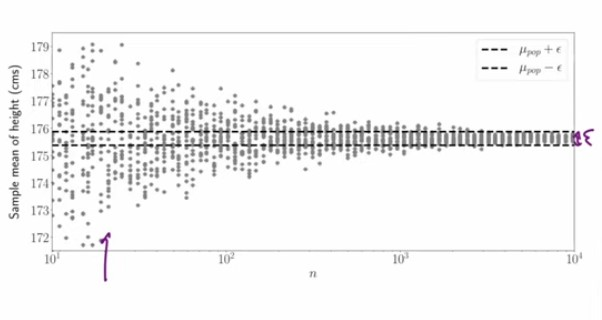
\includegraphics[width=10cm]{notes/week_3/Video 3:The Law of Large Numbers and Deviation Inequalities/immages/v_3_1.jpg}
\item so we can get bounds for probabilities using these bounds
\item we can see the law of large numbers 
\item and that the sample mean is constant so if we take enough samples the likelihood that our sample mean will differ from the population mean by any constant will approach 0
\item 
\end{itemize}
\end{document}
